\documentclass{article} % For LaTeX2e
\usepackage{nips14submit_e,times}
\usepackage{hyperref}
\usepackage{url}
\usepackage{graphicx}
%\documentstyle[nips14submit_09,times,art10]{article} % For LaTeX 2.09

\title{Identifying read words using images of brain activity : Milestone}


\author{
Tomasz Sarkedja \\
Physics Department\\
University of Washington\\
\texttt{email} \\
\And
Stella Stylianidou \\
Physics Department\\
University of Washington\\
\texttt{stellast@uw.edu} \\
}


\newcommand{\fix}{\marginpar{FIX}}
\newcommand{\new}{\marginpar{NEW}}

\nipsfinalcopy % Uncomment for camera-ready version

\begin{document}


\maketitle

\begin{abstract}
We describe an algorithm to predict a word a participant is reading using brain activation patterns in their brain. We use linear regression with sh FMRI brain scan data taken while a participant was reading a word, and the relationship of each word with a set of 218 semantic features. To obtain the parameters that relate each semantic feature to each voxel in the brain images we used linear regression with shrinkage of the features (Lasso). Our initial experiments have a success rate of %. 

\end{abstract}

\section{Introduction}

Humans always sought to understand the brain better. Functional magnetic resonance imaging (FMRI), which is an imaging procedure that measures brain activity by detecting changes associated with blood flow, has been a vital component in medical diagnosis but also in the process of improving our understanding of human brain and biology. The information hidden in an FMRI scan is though complicated and dense and only highly experts practitioners are able to decipher it. With the development of machine learning it is now possible to find relationships between FMRI scans and human actions or thoughts that were not possible before.

In this work we seek to find a relationship between FMRI scans and semantic features, the aspects that characterize a word. We then use the mappings between words and semantic features to find the word closest in distance to the predicted semantic features. Our data consisted of 60 words, and their relationship to the 216 semantic features, for which the values were centered around 0 and standardized. Furthermore, we had 360 FMRI images consisting of 20,000 voxels, each with a value for the brightness of the voxels, also standardized. Each semantic feature had to be separately related to the brightness of the voxels. 


\section{Methods}
\label{gen_inst}
Because FMRI scans are expensive the amount of data one can obtain is limited. This makes training our model difficult, since amount of training data (360) is significantly smaller than  the dimensions of the problem (20,000 voxels). To face this, we used linear linear regression with shrinkage of the features (Lasso).




\subsection{Lasso}

To obtain the parameters that relate the value of a semantic feature to the voxels in the brain images we used Lasso. Lasso,  adescribed in Tibshirani (1996), constrains the L1 norm, therefore shrinking some of the coefficients to exactly zero. This technique therefore obtains sparse solution, which can be useful in the cases that the amount of data is much smaller than the dimensions as in this case, or if we expect that few voxels are related to each word. 

Lasso estimates of the coefficients (Tibshirani, 1996) achieve minβ(Y−Xβ)′(Y−Xβ)+λ∑pj=1|βj|, so that the L2 penalty of ridge regression ∑pj=1β2j is replaced by an L1 penalty, ∑pj=1|βj|. Let c0=∑pj=1|β̂ LS,j| denote the absolute size of the least squares estimates. Values of 0<c<c0 cause shrinkage towards zero.


\section{Results}


\subsection{Obtaining the best lambda}
Since our dataset consists of only 300 FMRI images, we first attempted to choose the best lambda for our dataset using only one of the semantic features. 250 FMRI images were used to train our dataset and 50 were used as validation data to choose the lambda that minimizes the Root Mean Squared Error on that dataset. We started from maximum lambda calculated as $2 * max (|X^T.(y - <y>)|)$ and decreased the lambda by multiplying with 0.8 in each iteration. Choosing the lambda using this method on different semantic features obtained similar values for all features, but larger values than expected (~134). In figure 1, it is shown the root mean square error on the training data and validation data versus different lambdas. This creates a very sparse solution and setting most of the features to 0. The reason behind the large values of lambda may be due to the nature of the data, or the large dimensionality compared to the amount of training data we have.



\begin{figure}[h]
\begin{center}
%\framebox[4.0in]{$\;$}
%\fbox{\rule[-.5cm]{0cm}{4cm} \rule[-.5cm]{4cm}{0cm}}
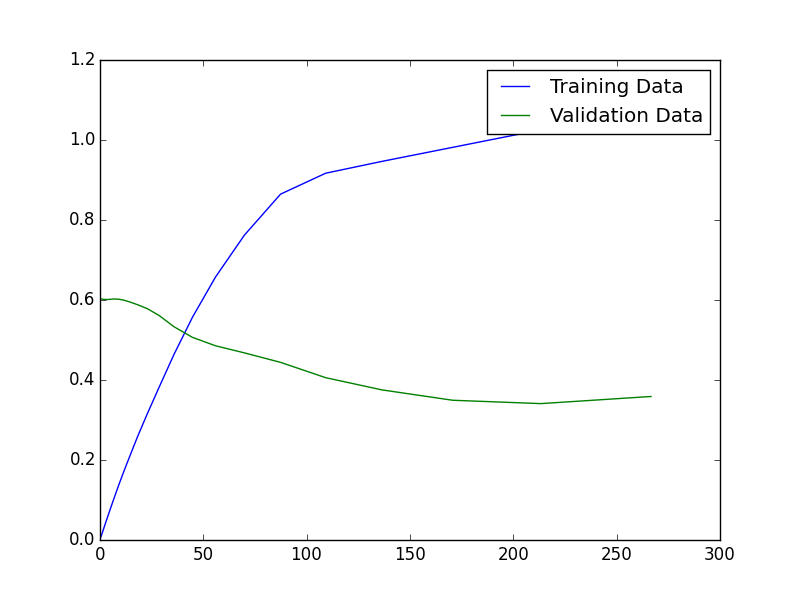
\includegraphics[scale=0.5]{trainvalidlambda}
\end{center}
\caption{Training lambdas on the first semantic feature on 250 data, and using 50 FMRI images as a validation test.}
\end{figure}

\subsection{Results on the test data}

Using the lambda above (134) which was obtained from training on the first feature,  we trained for each semantic feature for lambda 134 +/- 5 and choose the value with least RMSE square error on the validation set. With the obtained weights we predict the values for the 216 semantic features. The predicted semantic feature values are then compared to the semantic features of the two given words. The word of which the semantic features have the smallest distance from the predicted semantic features is chosen. 

For lambdas around 134 our results were close to random with only 52\% of the words guessed correctly (31 out of 60), indicating that the weights predicted are not satisfactory for the prediction of the semantic features.

We also run our algorithm with the lambdas suggested in the CSE599 homework where the data are from (0.05,0.1,0.15,0.2,0.25,0.3,0.35,0.4), but again obtained results a bit lower than random with 49\% of the words guessed correctly.


\section{Future Directions}


\subsection{Principal Component Analysis}
The difficulties with this problem is that our dimensionality is multiple times higher than the amount of data we have. A possible way to decrease our dimensions is to use Principal Component Analysis(PCA).  Principal Component Analysis transforms the set of observations that may be correlated into a a new basis where the set of values are linearly uncorrelated.



\subsubsection*{References}

\small{
%original lasso paper
Tibshirani, R. (1996). Regression shrinkage and selection via the lasso. J. Royal. Statist. Soc B., Vol. 58, No. 1, pages 267-288

%do pathwise optimization. This means starting with a high value for λ, solve the optimization for a decreasing sequence of lambdas using the previous results as a warm start.
Friedman, J., Hastie, T., \& Tibshirani, R. (2010). Regularization paths for generalized linear models via coordinate descent. Journal of statistical software, 33(1), 1.
%shooting
Wenjiang Fu (1998). Penalized regressions: the bridge vs the lasso. JCGS vol 7, no. 3, 397-416.
}

\end{document}
